\chapterauthor{Karl Thyssen}
Here we will discuss the results we saw for the various approaches we attempted.

As previously mentioned we experimented with a $\gamma$ value of $1.0$ and $0.9$ after which we continued other variations at $\gamma = 0.9$.
Other variations include:
\begin{itemize}
	\item $\gamma = 1.0$:
	\begin{itemize}
		\item Generation 0 data generated from 4 $\code{simple\_agents}$
		\begin{itemize}
			\item Additionally train MLB
		\end{itemize}
	\end{itemize}
	\item $\gamma = 0.9$:
	\begin{itemize}
		\item Generation 0 data generated from 4 $\code{simple\_agents}$:
		\begin{itemize}
			\item self-train until agents begin to regularly interact with each other
			\item self-train
			\item state vector reduced to 180 elements
		\end{itemize}
		\item Generation 0 data generated from 4 $\code{random\_agents}$:
		\begin{itemize}
			\item self-train until agents begin to regularly interact with each other
			\item self-train
		\end{itemize}
	\end{itemize}
\end{itemize}

%Discuss reasons behind initial approach - also mlp regressor (slow to fit so less data)
\subsection{The initial approach}

Having decided on the random forest regressors as the medium for storing our Q, and knowing the random forest has the ability to determine feature importances and weightings itself we decided to throw every feature we could think at it as described in \ref{State_rep}. We initially also chose a $\gamma$ value of $1.0$ for simplicity in testing and began to train an agent. In \cite{paper} the agent trains for 10000 episodes per generation and begins to show a large improvement between generations $10$ and $20$, however that agent is trained using a neural network so we expected a longer wait before seeing such spikes in performance. This is due to the erratic nature of the predictions made by the forests in relation to the MLP we tested.

Out of interest we also tested the same set-up using an MLP regressor, however unlike the forest, the impact of using any and all features was an exorbitant time required for the fitting after each generation, often longer than the data generation itself.

The average time required to generate data for and fit each generation was roughly $4800 seconds$. This time required is clearly dependent not only on hardware and thinking time but also the number of steps the agent takes per episode which was unfortunately consistently short.

\begin{figure}[h]
\centering
	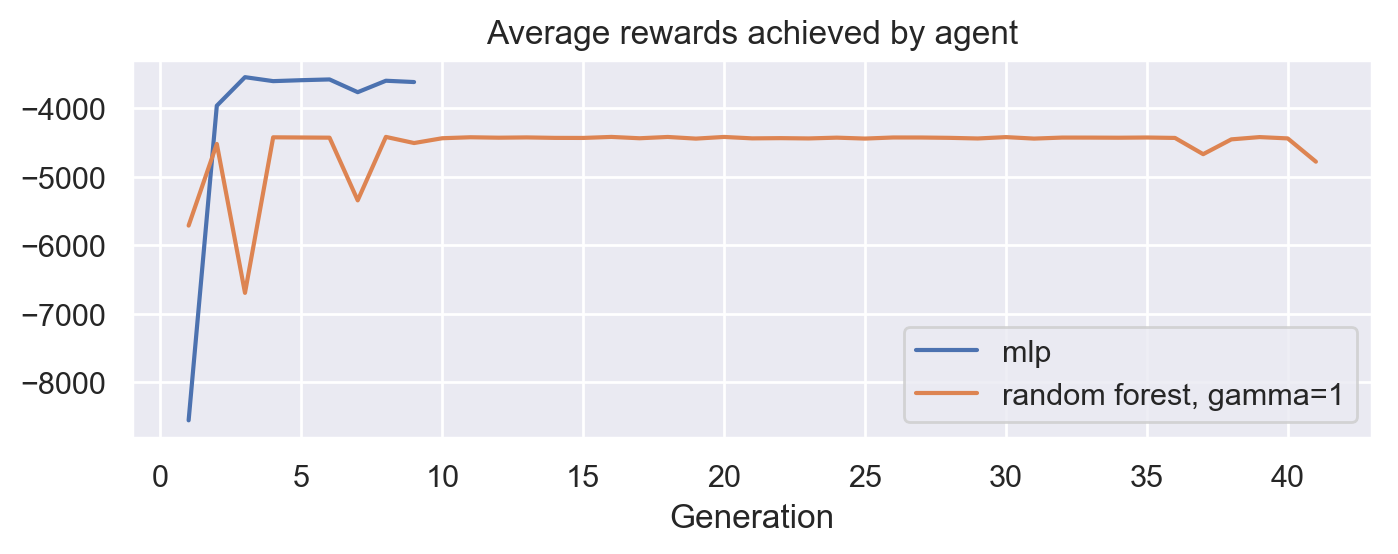
\includegraphics[width=\linewidth]{images/mlp_vs_forest_gamma_1.png}
	\caption{Here we see the performance of 40 generations trained with the random forest and 8 generations using the MLP. We chose not to train the MLP further as the time constraints were too severe and we were not seeing any improvement.}
	\label{mlp_vs_forest_gamma_1.0}
\end{figure}


%show results of initial training
%random forest too erratic - as single steps can be fatal, inaccuracies can have drastic consequences
%let train for a long time as unclear when we should see results
%present variations
%discuss changes and possible solutions - even fewer features, other machine learning methods

\subsection{Outlook}
\chapterauthor{Hein-Erik Schnell, Karl Thyssen}
As discussed in the previous subsection, our agents are very unsuccessful. They mostly remain in their starting corner and more often than not they blow themselves up. It is therefore necessary to discuss alternative approaches to the task and how we could have improved our implemented approaches.\par

% More time, maybe they would have learned then -> more episodes per generation, more generations in general
% Exploration/Exploitation
% Much smaller state vector, no representation of the whole board
% Different initial settings of regressors
% Update regressors, not refit
% Different reward scheme, other gamma

As we see it, the topics to be discussed are mostly the sections above:
\begin{itemize}
	\item State representation
	\item Reward scheme
	\item Regressors
	\item Training procedure
	\item Exploration / Exploitation
\end{itemize}

\subsubsection{State Representation}
With what we saw so far, we have to assume that less features in the state vector lead to far less possible states and better performance of the agent. The $180$-features version of the state vector is already close to the smallest form of state vector possible if we want to represent the whole game board, which would be at least $176$ features ($176$ accessible cells). \par
A possible improvement would be a state vector which does not represent the whole game board. The simple agents, for example, only know the position of possible targets and whether they are in danger. With this in mind, we could create a state vector which gives only the informations relevant to the simple agents. Given that in most cases most of the game board is not relevant (especially at the beginning of an episode), this seems to be a quite reasonable approach. It would also help the agent to prioritize certain features, e.g. avoid explosions before collecting coins.

\subsubsection{Reward Scheme}
In the plots above, we see that achieved scores and rewards hardly correlate. In the ideal case, higher score means more rewards. Since this is not the case, we need to revisit our reward scheme and distribute much higher rewards for what actually scores. On the other hand, our agent died a lot which meant lots of penalties. But we don't get negative scores for dying. We don't really know which way is better and we would have tried both ways in order to find out.

\subsubsection{Regressors}
The regressors were the third crucial design choice. As hinted above, choosing a regressor which is very erratic (Random Forest Regressor) and one which we don't know much about (MLP-Regressor) left us somewhat dissatisfied. Still, they were the most practical choices to us.\par
For both regressors we used almost the default settings. Adjusting those settings accordingly to our task might have helped a lot. But in the case of the MLP-Regressor, we could only guess what effects the various parameters might have. \par

All in all, choosing a better suited regressor and adjusting its parameters properly are two of the most important tasks in order to improve our model.\par

One should also mention that, after each generation, we fitted a whole new Forest. One could try to adjust the former Forest towards the data, instead.

\subsubsection{Training procedure}
We mostly trained our model with $10000$ episodes per generation. In one case even for more than $40$ generations (i.e. $400000$ episodes). Since Reinforcement Learning sometimes requires long times before encountering a good policy, we could never know whether our agent is not able to learn properly (because of the points above) or if it just didn't have enough time. With almost no experience from prior projects or exercises concerning RL, we didn't know how to find out which is the case. Speaking of only the training procedure, having more episodes per generation and letting it run for more generations might always improve the results.

\subsubsection{Exploration / Exploitation}
As mentioned before, the agent tends to kill itself if \textit{exploration} is enabled because it is likely to take random actions shortly after having placed a bomb. In order to prevent this, one could lower the $\epsilon$ significantly. Apart from that, we think that \textit{exploration/exploitation} is of less importance in terms of improving the model. The bottleneck are the points mentioned in \textit{State Representation, Reward Scheme} and \textit{Regressors}. 

\subsection{Further Comments on the final project}
As already implied in several parts of the report, our greatest issue was the lack of knowledge and experience with Reinforcement Learning. Some exercises with feedback and sample solutions would have helped a lot. For the next time, I propose to divide the final project into subtasks which are then given to the students as the final one or two exercise sheets and let the final project be something like the final improvements to an already working environment and model.